% Options for packages loaded elsewhere
\PassOptionsToPackage{unicode}{hyperref}
\PassOptionsToPackage{hyphens}{url}
%
\documentclass[
]{article}
\usepackage{amsmath,amssymb}
\usepackage{lmodern}
\usepackage{iftex}
\ifPDFTeX
  \usepackage[T1]{fontenc}
  \usepackage[utf8]{inputenc}
  \usepackage{textcomp} % provide euro and other symbols
\else % if luatex or xetex
  \usepackage{unicode-math}
  \defaultfontfeatures{Scale=MatchLowercase}
  \defaultfontfeatures[\rmfamily]{Ligatures=TeX,Scale=1}
\fi
% Use upquote if available, for straight quotes in verbatim environments
\IfFileExists{upquote.sty}{\usepackage{upquote}}{}
\IfFileExists{microtype.sty}{% use microtype if available
  \usepackage[]{microtype}
  \UseMicrotypeSet[protrusion]{basicmath} % disable protrusion for tt fonts
}{}
\makeatletter
\@ifundefined{KOMAClassName}{% if non-KOMA class
  \IfFileExists{parskip.sty}{%
    \usepackage{parskip}
  }{% else
    \setlength{\parindent}{0pt}
    \setlength{\parskip}{6pt plus 2pt minus 1pt}}
}{% if KOMA class
  \KOMAoptions{parskip=half}}
\makeatother
\usepackage{xcolor}
\usepackage[margin=1in]{geometry}
\usepackage{graphicx}
\makeatletter
\def\maxwidth{\ifdim\Gin@nat@width>\linewidth\linewidth\else\Gin@nat@width\fi}
\def\maxheight{\ifdim\Gin@nat@height>\textheight\textheight\else\Gin@nat@height\fi}
\makeatother
% Scale images if necessary, so that they will not overflow the page
% margins by default, and it is still possible to overwrite the defaults
% using explicit options in \includegraphics[width, height, ...]{}
\setkeys{Gin}{width=\maxwidth,height=\maxheight,keepaspectratio}
% Set default figure placement to htbp
\makeatletter
\def\fps@figure{htbp}
\makeatother
\setlength{\emergencystretch}{3em} % prevent overfull lines
\providecommand{\tightlist}{%
  \setlength{\itemsep}{0pt}\setlength{\parskip}{0pt}}
\setcounter{secnumdepth}{-\maxdimen} % remove section numbering
\newlength{\cslhangindent}
\setlength{\cslhangindent}{1.5em}
\newlength{\csllabelwidth}
\setlength{\csllabelwidth}{3em}
\newlength{\cslentryspacingunit} % times entry-spacing
\setlength{\cslentryspacingunit}{\parskip}
\newenvironment{CSLReferences}[2] % #1 hanging-ident, #2 entry spacing
 {% don't indent paragraphs
  \setlength{\parindent}{0pt}
  % turn on hanging indent if param 1 is 1
  \ifodd #1
  \let\oldpar\par
  \def\par{\hangindent=\cslhangindent\oldpar}
  \fi
  % set entry spacing
  \setlength{\parskip}{#2\cslentryspacingunit}
 }%
 {}
\usepackage{calc}
\newcommand{\CSLBlock}[1]{#1\hfill\break}
\newcommand{\CSLLeftMargin}[1]{\parbox[t]{\csllabelwidth}{#1}}
\newcommand{\CSLRightInline}[1]{\parbox[t]{\linewidth - \csllabelwidth}{#1}\break}
\newcommand{\CSLIndent}[1]{\hspace{\cslhangindent}#1}
\usepackage{lineno}
\linenumbers
\usepackage{setspace}\doublespacing
\usepackage{gensymb}
\usepackage{caption}
\captionsetup[figure]{labelformat=empty}
\usepackage{float}
\ifLuaTeX
  \usepackage{selnolig}  % disable illegal ligatures
\fi
\IfFileExists{bookmark.sty}{\usepackage{bookmark}}{\usepackage{hyperref}}
\IfFileExists{xurl.sty}{\usepackage{xurl}}{} % add URL line breaks if available
\urlstyle{same} % disable monospaced font for URLs
\hypersetup{
  pdftitle={Quantifying Impacts of an Environmental Intervention Using Environmental DNA: Supplemental Text 2},
  pdfauthor={Elizabeth Andruszkiewicz Allan,; Ryan P. Kelly,; Erin D'Agnese,; Maya Garber-Yonts,; Megan Shaffer,; Zachary Gold,; Andrew O. Shelton},
  hidelinks,
  pdfcreator={LaTeX via pandoc}}

\title{Quantifying Impacts of an Environmental Intervention Using
Environmental DNA: Supplemental Text 2}
\author{Elizabeth Andruszkiewicz Allan, \and Ryan P. Kelly, \and Erin
D'Agnese, \and Maya Garber-Yonts, \and Megan Shaffer, \and Zachary
Gold, \and Andrew O. Shelton}
\date{2023}

\begin{document}
\maketitle

For submission to: \textit{Ecological Applications}

Our analysis depends upon a set of quantitative models, each linking our
observations of metabarcoding reads or qPCR cycle-threshold values to an
underlying concentration of target-species DNA in water samples.

In summary, we (1) use a mock community with a known composition to
calibrate our environmental metabarcoding data as described in (Shelton
et al. 2022). The result is a set of estimated proportions of DNA from
each species in each sample. We then (2) relate qPCR cycle-threshold
values for a reference species (here, cutthroat trout (\emph{O.
clarkii})) from the same set of samples to a standard curve to yield
quantitative estimates of the concentration of our reference species in
each sample. We (3) use these absolute estimates of DNA concentration to
expand the metabarcoding-derived proportion data into a complete set of
quantitative estimates of DNA concentrations for each species in each
sample. We account for the variable water-flow-rates of the sampled
creeks by converting these concentrations from units of copies/L into
units of copies/s, given an flow rate in L/s. Finally, we (4) construct
a model describing changes in these species-specific concentrations over
time. We give the statistical details of these steps below.

\hypertarget{calibration-with-a-mock-community}{%
\subsection{Calibration with a Mock
Community}\label{calibration-with-a-mock-community}}

See Shelton et al. (2022); McLaren et al. (2019); Silverman et al.
(2021) for similar analyses.

For ease of computation, we ran the metabarcoding-calibration model on
data for each of our five creeks separately, using the same mock
communities to calibrate each.

Model Diagnostics: 3 chains, 1500 iterations, for all parameters,
\(\hat{R} \leq 1.02\)

\hypertarget{qpcr-calibration}{%
\subsection{qPCR Calibration}\label{qpcr-calibration}}

See Shelton et al. (2019); McCall et al. (2014) for similar analyses.

For all samples \(i\), on qPCR plates \(j\), we either observe
(\(z_{i,j} = 0\) or do not observe \(z_{i,j} = 1\)) amplification; we
omit the subscripts \(i\) and \(j\) from the following description
except where necessary for clarity. We assume an intercept of zero.

We model the probability of detection \(P(z = 1)\)) as a linear function
of concentration and slope parameter \(\phi\),
(\(P(z = 1) = \theta = c\phi\)), with a logit transform to constrain the
inferred probability to between 0 and 1.

For those samples that amplify (\(z = 1\)), we model the observed Ct
value (\(y\)) as a linear function of our parameter of interest, the
log-concentration of target-species DNA under analysis (\(c\)). We treat
\(y\) as drawn from a normal distribution
\(y \sim N(\mu_{i,j}, \sigma_{i,j})\)), where each triplicate sample on
each qPCR plate has its own estimated mean and standard deviation. The
means are estimated as a straightforward linear model,
\(\mu = \beta_{0,j} + \beta_{1,j}c\), but we allow the standard
deviation to vary as a linear function of log-concentration so as to
accurately capture decreasing precision with decreasing concentration:
\(\sigma = e^{\gamma_{0} + \gamma_{1,j}c}\); we estimate these
parameters as an exponent to constrain \(\sigma > 0\).

Samples with known concentrations (i.e., standards) were fit jointly
with unknown samples (i.e., environmental samples); because qPCR plate
identity was shared among all environmental samples and standards within
a plate, this has the effect of applying plate-specific slope and
intercept values for the standard curve to each of the environmental
samples on the plate (Figure S13).

We apply moderately informative priors that make use of background
information in hand. For example, because qPCR standard curves of all
kinds have slopes near -3, this slope becomes our background expectation
as embodied in the prior on \(\beta_1\), but the standard deviation of
that prior leaves plenty of room for this background to be overwhelmed
by the observed data. The same logic applies to the intercept of the
standard curve, which in qPCR (for any given species) generally falls
near 39 cycles, an expectation that we formalize by having \(\beta_0\)
drawn from a normal distribution with \(\mu = 39\) and \(\sigma = 3\).

Taken together with priors, the model is:

\begin{gather*}
z_{i,j} \sim Bernoulli(\theta_{i,j}) \\
\theta_{i,j} = logit^{-1}(\phi c_{i,j}) \\[4mm]
y_{i,j} \sim Normal(\mu_{i,j}, \sigma_{i,j})   \text{    if } z_{i,j} = 1 \\
\mu_{i,j} = \beta_{0,j} + \beta_{1,j} c_{i,j} \\
\sigma_{i,j} = e^{\gamma_{0}  + \gamma_{1,j} c_{i,j}} \\[4mm]
\beta_{0} \sim normal(39, 3) \\
\beta_{1} \sim normal(-3, 1) \\
\gamma_{1} \sim normal(0,5) \\
\gamma_{0} \sim normal(-2,1)
\end{gather*}

\begin{figure}
\centering
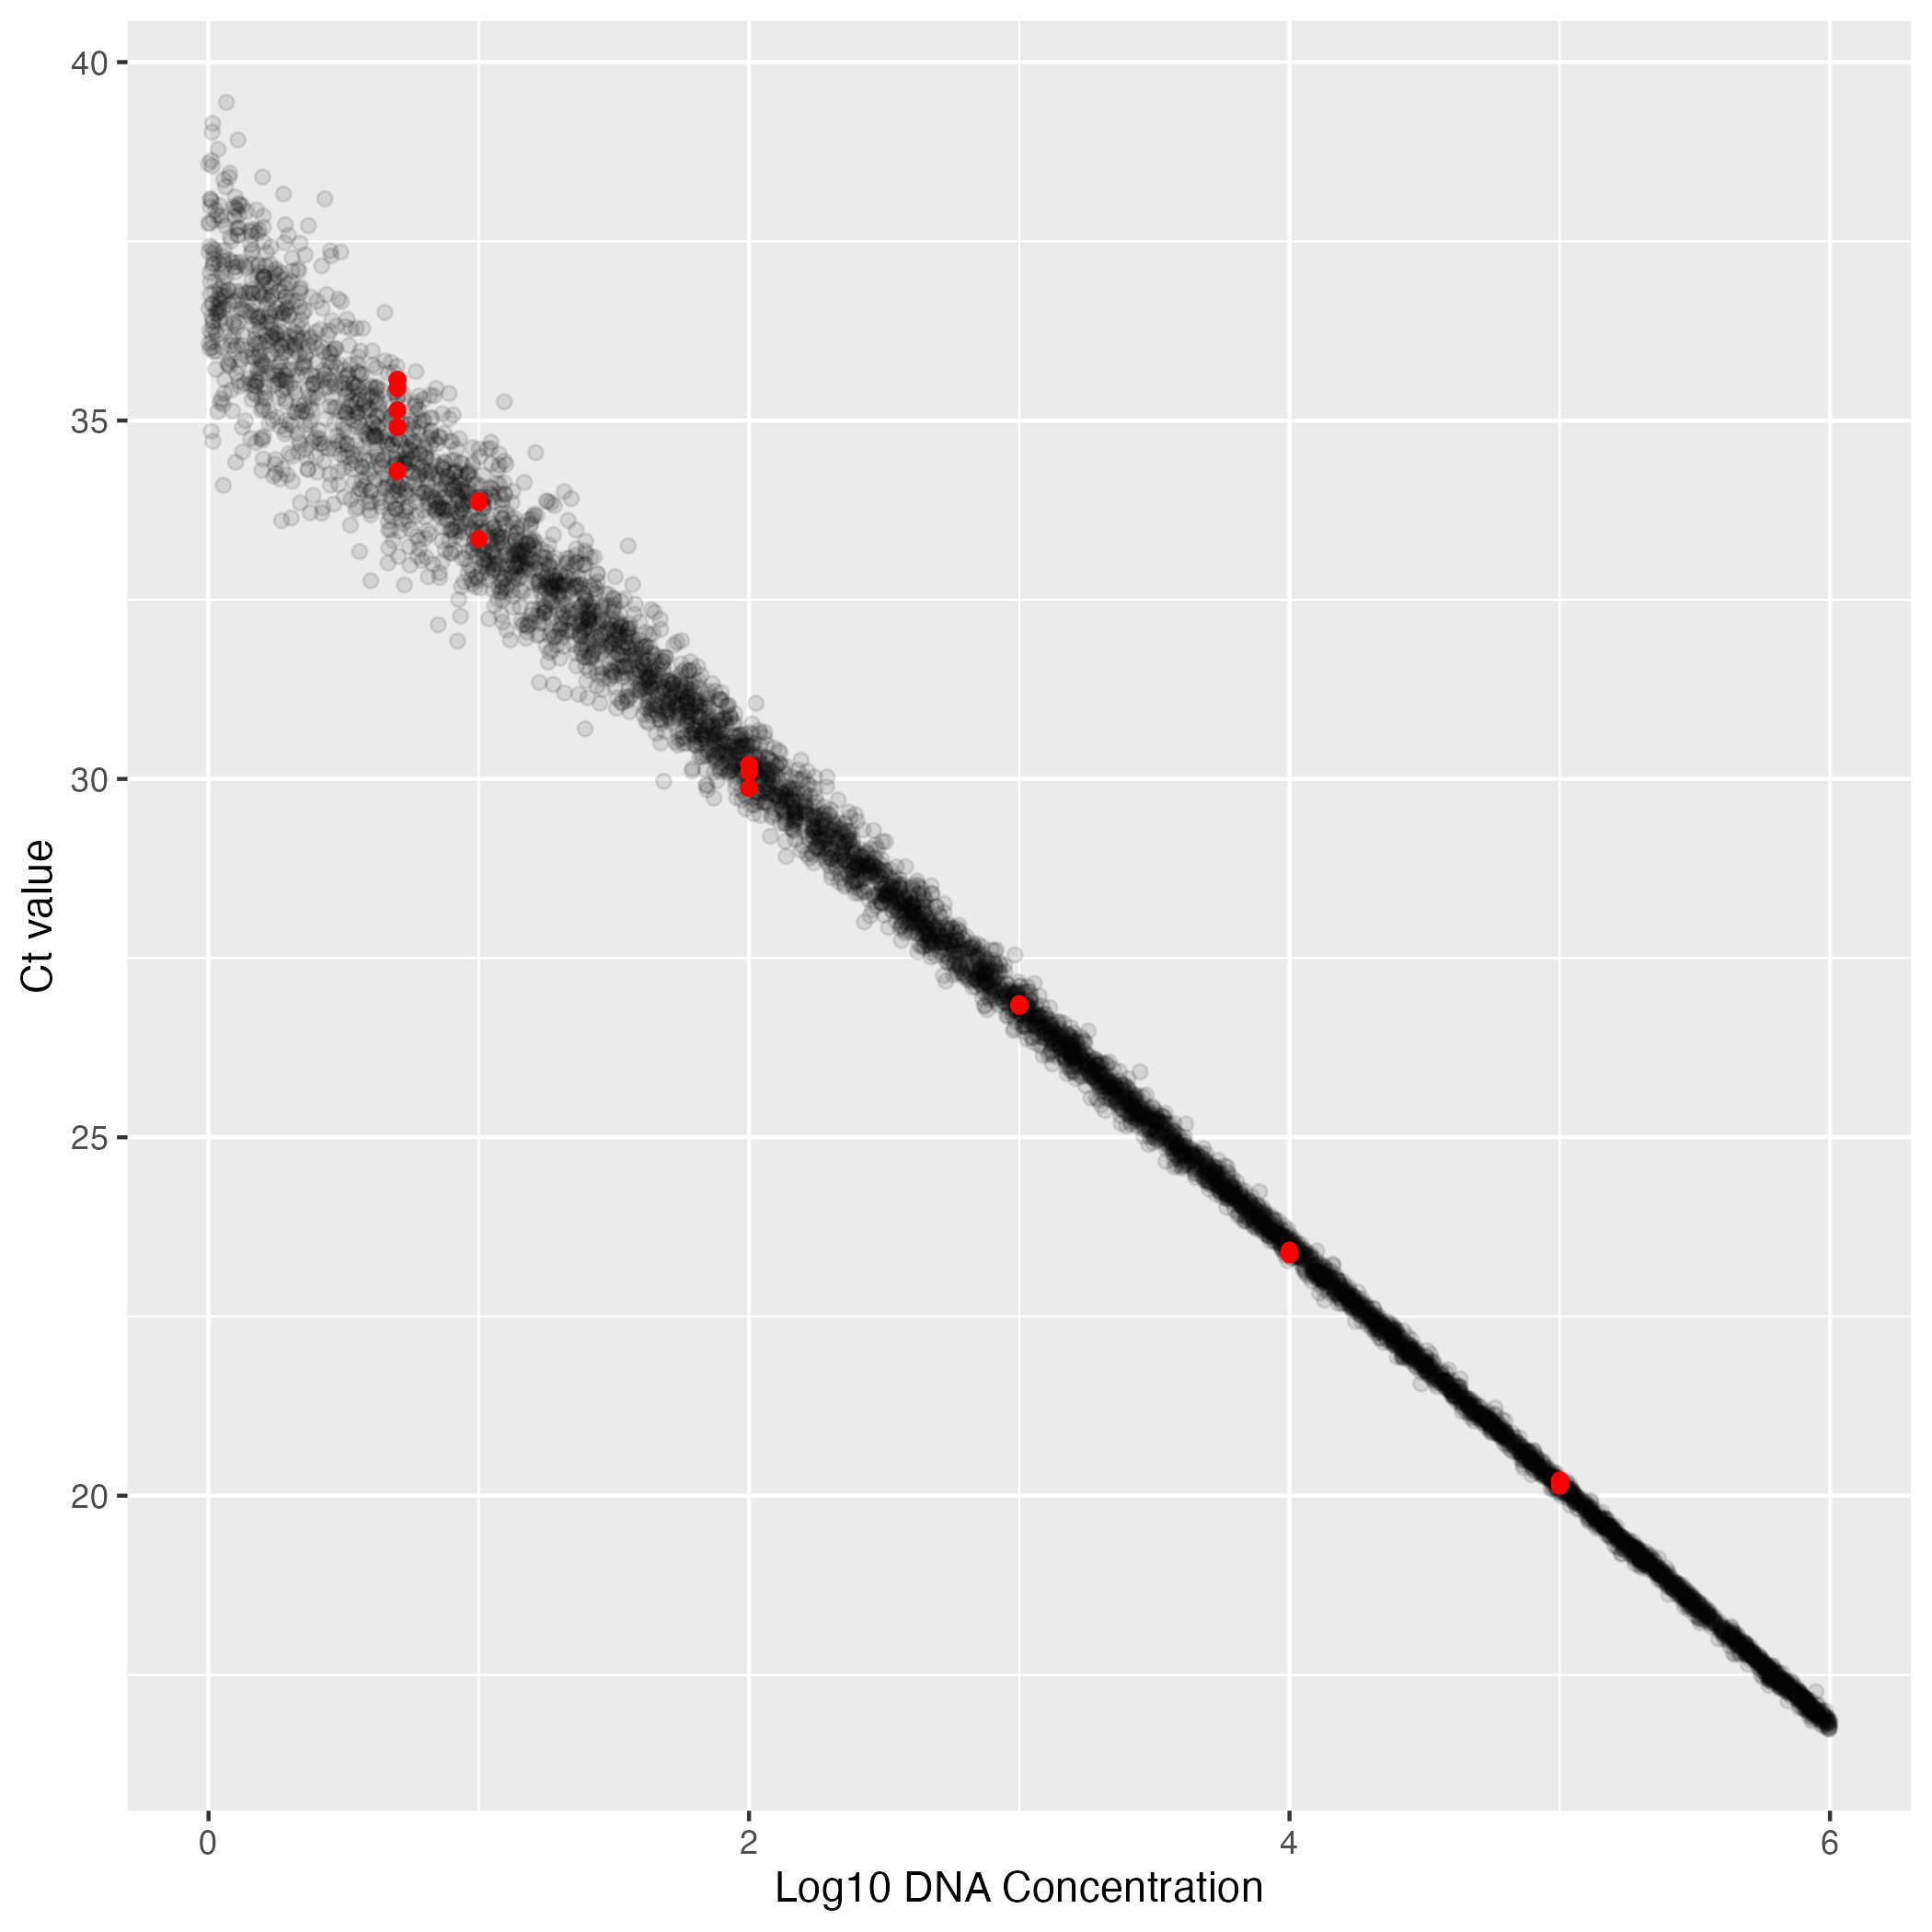
\includegraphics{../Output/SupplementalFigures/qPCR_calibration_supplemental.png}
\caption{Figure S13. Example of 2500 samples from the joint posterior
distribution of the model fit for a single representative qPCR plate.
Red dots are standard-curve observations with known starting
concentrations. The spread of black dots (posterior samples) indicates
the shape of the calibration curve, with standard deviation increasing
as concentration decreases.\label{fig:qpcrmodel}}
\end{figure}

Model Diagnostics: 3 chains, 2500 iterations, for all parameters,
\(\hat{R} \leq 1.002\).

\hypertarget{expanding-proportions-into-absolute-abundances}{%
\subsection{Expanding Proportions into Absolute
Abundances}\label{expanding-proportions-into-absolute-abundances}}

See Pont et al. (2022) and McLaren et al. (n.d.) (preprint) for examples
of similar expansions.

As described in the main text, calibrated metabarcoding analysis yielded
quantitative estimates of the proportions of species' DNA in
environmental samples prior to PCR.

We then converted these proportions into absolute abundances by
expansion, in light of the qPCR results for our reference species
\emph{O. clarkii}. We estimated the total amplifiable salmonid DNA in
environmental sample \(i\) as
\(DNA_{salmonid_{i}} = \frac{[qPCR_{reference_{i}}]}{Proportion_{reference_{i}}}\),
and then expanded species' proportions into absolute concentrations by
multiplying these sample-specific total concentrations by individual
species' proportions, such that for species \(j\) in sample \(i\),
\(DNA_{i,j} = DNA_{salmonid_{i}} * Proportion_{i,j}\).

We transformed the resulting abundances to account for the creeks'
flow-rates as described in the main text.

Ideally, we would have fit a joint model that simultaneously estimated
species proportions (metabarcoding), absolute concentrations (qPCR), and
developed the time-series trends for all species. As a practical
computational matter, we had to create these models individually, which
entailed some loss of information about parameter variability and cross
correlation. For the mixed-effects model describing trends over time
(described below), we used the product of posterior means from the
metabarcoding and the concentrations of the qPCR model as observations,
rather than being able to use the full posteriors for each input to the
model. We deemed this acceptable because our metabarcoding proportions
were quite precisely estimated: for example, in our focal Padden Creek,
the coefficient of variation for estimated proportions of our reference
species (\emph{O. clarkii}) ranged from 0.008 to 0.25.

\hypertarget{modeling-changes-in-concentration-over-time}{%
\subsection{Modeling Changes in Concentration over
Time}\label{modeling-changes-in-concentration-over-time}}

At a given station in a given creek, some DNA concentration exists for
each species. For simplicity, we focus on a single species and a single
station (downstream or upstream) for the moment.

Our observations of the (log) DNA concentration in creek \(i\) at time
\(t\) are distributed as
\(Y_{i,t} \sim \mathcal{N}(\mu_{i,t},\,\sigma^{2})\). More complex
versions of the model may let \(\sigma\) vary across creeks, time
points, species, or with environmental covariates of interest.

We are interested in how the DNA concentration changes over time, so we
model the expected value of DNA in a creek at time \(t\), \(\mu_{i,t}\).

We considered three ways of modeling the salmonid eDNA data, each in a
Bayesian framework, but each treating non-independence among time points
somewhat differently:

\begin{itemize}
\tightlist
\item
  A linear auto-regressive (AR(1)) model, written in \texttt{stan}. For
  each species in each creek, the expected concentration of eDNA of each
  month is a linear function of the expected value from the previous
  month. Within a species, the monthly autoregressive parameters are
  shared across creeks. For each species \(j\) -- the subscript for
  which we omit here for clarity -- we have a single overall model of
  the change in eDNA concentration among species, creeks (\(i\)),
  timepoints (\(t\)), and stations (\(d\)).
\end{itemize}

\begin{align*}
&Y_{i,t,d} \sim \mathcal{N}(\mu_{i,t,d},\,\sigma_{\text{obs}}^{2})\\
&\mu_{i,t,d} = \alpha_{i,t} + \epsilon_{i,t,d} + \eta_{i,t,d}\\
&\epsilon_{i,t,d} \sim \mathcal{N}(\beta\mu_{i,t-1,d},\, \phi^2)\\
&\alpha_{i,t} \sim \mathcal{N}(\mu_{\alpha}, \sigma_{\alpha})\\
&\beta \sim \mathcal{U}(-1, 1) \\
&\sigma_{\text{obs}} \sim gamma(1,2) \\
&\sigma_{\alpha} \sim gamma(1,2) \\
&\eta \sim \mathcal{N}(\mu_{\eta}, 1) \\
&\phi \sim gamma(1,2) \\
&\bf{\mu_{\alpha}} \sim \mathcal{N}(0, 10) \\
&\bf{\mu_{\alpha}} \sim \mathcal{N}(0, 5)
\end{align*}

\begin{itemize}
\tightlist
\item
  A generalized additive model (GAM), written in \texttt{brms} (which
  itself writes a \texttt{stan} model). For each species in each creek,
  an independent set of spline (weighting) parameters describes the
  temporal trends in expected eDNA concentration; the number of spline
  knots is shared across species and creeks. We follow (Pedersen et al.
  2019) to create a hierarchical GAM in which the expected value for
  each species in each creek at each time point is a spline function of
  time, time-by-creek, and time-by-station, with random effects for
  creek and station. Here, time-by-creek and time-by-station splines are
  centered, requiring additional fixed-effect terms for station and
  creek. Because no information is shared across species in this model,
  we fit the model each species independently.
\end{itemize}

\[\mu_{idt} = \beta_0 + s(t) + s_{d}(t) + s_{i}(t) + s(d) + s(i) \]

In \texttt{R} code using \texttt{brms}, this model is coded as

\begin{verbatim}
brm(
  bf(
    log(observed) ~ 
               s(time_idx, bs="cc") + 
               s(time_idx, by=station, m=1, bs="cc")+  #main effect, station
               s(station, bs="re") +  #random effect, station
               s(time_idx, by=creek, m=1, bs="cc")+  #main effect, creek
               s(creek, bs="re") + #random effect, creek
  )
)
\end{verbatim}

\begin{itemize}
\tightlist
\item
  A linear mixed-effects (LME) model, written in \texttt{rstanarm}. For
  each species in each creek, time (i.e., sampling month) is treated as
  a random effect. Each species-creek-month effect is treated as an
  independent draw from a common distribution.
\end{itemize}

\[\mu_{ijdt} = \beta_0 + \beta_{1_{ij}} + Month*\beta_{2_{ij}} + \beta_{3_{ijdt}}\]

In \texttt{R} code using \texttt{rstanarm}, this model is coded as

\begin{verbatim}
stan_glmer(log(observed) ~ (1 + time_idx|creek:species) + (1|station:creek:species:time_idx)
\end{verbatim}

Ultimately, the three models yielded very similar results (Figure S14).
The LME model proved simplest and most flexible insofar as it could
easily handle datasets with uneven sets of observations -- for example,
cases in which a species was detected downstream of a barrier, but not
upstream. We accordingly used the LME as the model for the analysis
given in the main manuscript.

\begin{figure}
\centering
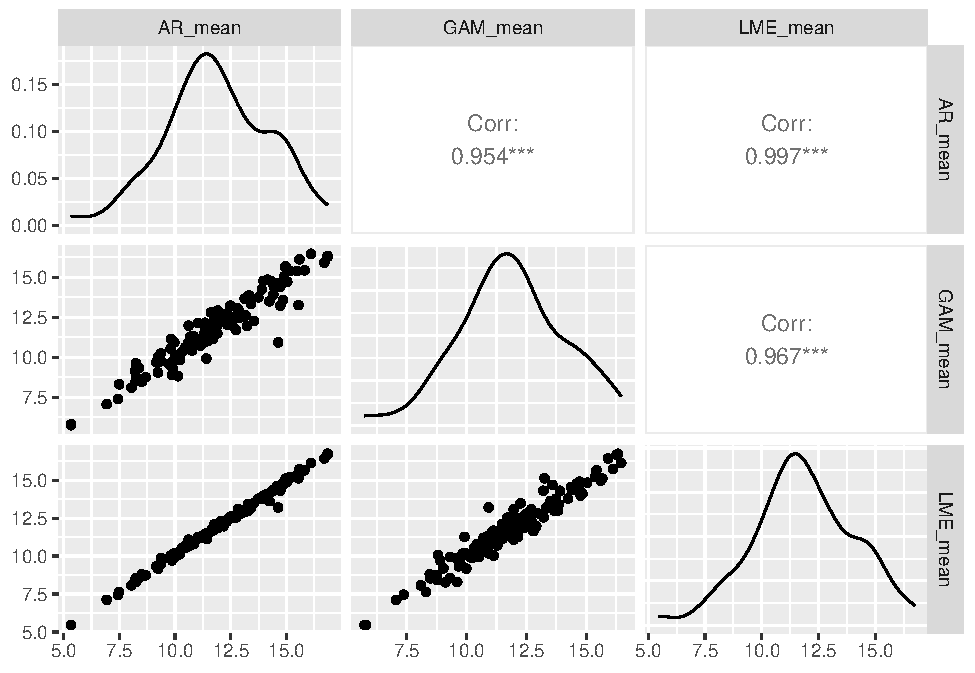
\includegraphics{../Output/SupplementalFigures/stats_comparisonplot.pdf}
\caption{Figure S14. Comparison of three models (linear autoregressive,
generalized additive model, and linear mixed effects model) shown for a
subset of the data used in the main
manuscript.\label{fig:comparemodels}}
\end{figure}

\newpage

\hypertarget{references}{%
\subsection*{References}\label{references}}
\addcontentsline{toc}{subsection}{References}

\hypertarget{refs}{}
\begin{CSLReferences}{1}{0}
\leavevmode\vadjust pre{\hypertarget{ref-mccall2014}{}}%
McCall, M. N., H. R. McMurray, H. Land, and A. Almudevar. 2014.
\href{https://doi.org/10.1093/bioinformatics/btu239}{On non-detects in
qPCR data}. Bioinformatics 30:2310--2316.

\leavevmode\vadjust pre{\hypertarget{ref-mclaren}{}}%
McLaren, M. R., J. T. Nearing, A. D. Willis, K. G. Lloyd, and B. J.
Callahan. (n.d.).
\href{https://doi.org/10.1101/2022.08.19.504330}{Implications of
taxonomic bias for microbial differential-abundance analysis}.

\leavevmode\vadjust pre{\hypertarget{ref-mclaren2019}{}}%
McLaren, M. R., A. D. Willis, and B. J. Callahan. 2019.
\href{https://doi.org/10.7554/eLife.46923}{Consistent and correctable
bias in metagenomic sequencing experiments}. eLife 8:e46923.

\leavevmode\vadjust pre{\hypertarget{ref-pedersen2019}{}}%
Pedersen, E. J., D. L. Miller, G. L. Simpson, and N. Ross. 2019.
\href{https://doi.org/10.7717/peerj.6876}{Hierarchical generalized
additive models in ecology: an introduction with mgcv}. PeerJ 7:e6876.

\leavevmode\vadjust pre{\hypertarget{ref-pont2022a}{}}%
Pont, D., P. Meulenbroek, V. Bammer, T. Dejean, T. Erős, P. Jean, M.
Lenhardt, C. Nagel, L. Pekarik, M. Schabuss, B. C. Stoeckle, E. Stoica,
H. Zornig, A. Weigand, and A. Valentini. 2022.
\href{https://doi.org/10.1111/1755-0998.13715}{Quantitative monitoring
of diverse fish communities on a large scale combining eDNA
metabarcoding and qPCR}. Molecular Ecology Resources n/a.

\leavevmode\vadjust pre{\hypertarget{ref-shelton}{}}%
Shelton, A. O., Z. J. Gold, A. J. Jensen, E. D'Agnese, E. Andruszkiewicz
Allan, A. Van Cise, R. Gallego, A. Ramón-Laca, M. Garber-Yonts, K.
Parsons, and R. P. Kelly. 2022.
\href{https://doi.org/10.1002/ecy.3906}{Toward quantitative
metabarcoding}. Ecology n/a:e3906.

\leavevmode\vadjust pre{\hypertarget{ref-shelton2019}{}}%
Shelton, A. O., R. P. Kelly, J. L. O'Donnell, L. Park, P. Schwenke, C.
Greene, R. A. Henderson, and E. M. Beamer. 2019.
\href{https://doi.org/10.1016/j.biocon.2019.07.003}{Environmental DNA
provides quantitative estimates of a threatened salmon species}.
Biological Conservation 237:383--391.

\leavevmode\vadjust pre{\hypertarget{ref-silverman2021}{}}%
Silverman, J. D., R. J. Bloom, S. Jiang, H. K. Durand, E. Dallow, S.
Mukherjee, and L. A. David. 2021.
\href{https://doi.org/10.1371/journal.pcbi.1009113}{Measuring and
mitigating PCR bias in microbiota datasets}. PLoS Computational Biology
17:e1009113.

\end{CSLReferences}

\end{document}
